\documentclass[aspectratio=169]{beamer}
\usepackage{graphicx} % Required for inserting images
\usepackage[
backend=biber,
style=numeric,
sorting=ynt]{biblatex}
\usepackage{chngcntr}
\counterwithin{figure}{section}
\usetheme{CambridgeUS}
\usecolortheme{beaver}
\addbibresource{ref.bib}
\title{Prison Management System}
\author{Nihar Niranjan S \and Nikith T Rajan \and Niranjay Ajayan \and Varun Raj R}
\institute{
	Department of Computer Engineering\\
	Model Engineering College\\
	Thrikkakara, Kochi 682021\\
}
\begin{document}
\begin{frame}[plain]
    \maketitle
\end{frame}
\begin{frame}{Table Of Contents}
    \tableofcontents
    
\end{frame}
\section{Introduction}
\begin{frame}
    \frametitle{Introduction}
    \begin{itemize}
        \item The Prison Management System (PMS) modernizes prison administration with a state-of-the-art solution.
        \item Traditional manual record-keeping methods in correctional facilities often lead to errors, inefficiency, and security risks.
        \item PMS eliminates the need for manual processes by transitioning them to a secure, centralized, and user-friendly platform.
        \item Significant improvements are achieved in the following areas:
        \begin{itemize}
            \item Accuracy: Reduces the likelihood of human errors in record keeping.
            \item Efficiency: Streamlines day-to-day operations, making them faster and more organized.
            \item Security: Enhances safety for both inmates and prison staff by maintaining better control over sensitive data.
        \end{itemize}
    \end{itemize}
\end{frame}
\section{SRS}
\subsection{Functional Requirements}
\begin{frame}{Functional Requirements}
    \textbf{Staff Management}
    \begin{itemize}
        \item Login: Staff can securely log in using their staff ID and password.
        \item View/Manage Staff: Ability to view, register, update roles, or remove staff members.
    \end{itemize}
    \textbf{Prisoner Management}
    \begin{itemize}
        \item Add/Release Prisoners: Functions to add new prisoners and release them when required.
        \item Update Prisoner Information: Modify prisoner details, including reassignment to cells.
        \item Generate Prisoner Reports: Access comprehensive information on prisoners.
    \end{itemize}   
    
\end{frame}
\begin{frame}{Functional Requirements}
    \textbf{Cell and Task Management}
    \begin{itemize}
        \item Allocate/Change Cells: Assign prisoners to cells or reassign them.
        \item Assign/Record Work: Assign jobs to prisoners and track their work hours

    \end{itemize}
    \textbf{Visitor and Incident Tracking}
    \begin{itemize}
        \item  Register a new visitor and keep the visitors history
        \item Filter the records of prisoners by crime and generate statistics on the type of crime
    \end{itemize}
    
\end{frame}
\begin{frame}{Functional Requirements}
    \begin{itemize}
        \item \textbf{Frontend:} The user interface is built using React and styled with CSS, making it responsive and easy to navigate. This ensures users can interact with the system smoothly, whether on desktop or mobile.
        \item \textbf{Backend:} Python powers the backend, managing all the logic and API communication to keep everything running efficiently behind the scenes.
        \item \textbf{Database:} MySQL is used to securely store all critical data, including prisoners, staff, and visitors.
        \item \textbf{Security:} For added safety, hashlib encrypts sensitive information, ensuring data integrity and secure access.
    \end{itemize}
\end{frame}
\subsection{Non-Functional Requirements}
\begin{frame}{Non-Functional Requirements}
    \textbf{Performance Requirements}
    \begin{itemize}
        \item Handle access by multiple staff users 
        \item Quick data retrieval 
    \end{itemize}
    \textbf{Security Requirements}
    \begin{itemize}
        \item Ensure role-based access control for staff roles (admin, staff)
        \item Encrypt sensitive data (e.g., login credentials) using secure hashing techniques like hashlib.
    \end{itemize}
    \textbf{Usability Requirements}
    \begin{itemize}
        \item User-friendly React-based interface with smooth navigation.
        \item Mobile-responsive design using CSS
    \end{itemize}
    
\end{frame}
\section{Architecture}
\subsection{Architecture Description}
\begin{frame}{Architecture Description}
    \begin{itemize}
        \item The prison management system is a modular, multi-functional system divided into subsystems that manage various aspects of the prison, such as staff, prisoners, cells, tasks, visitors, and crime tracking. 
        \item Each subsystem handles a specific set of responsibilities, allowing for seamless coordination between them to achieve the overall functionality.\cite{designdoc}
    \end{itemize}
\end{frame}
\subsection{UML Diagrams}
\begin{frame}{}
    \begin{figure}
        \centering
        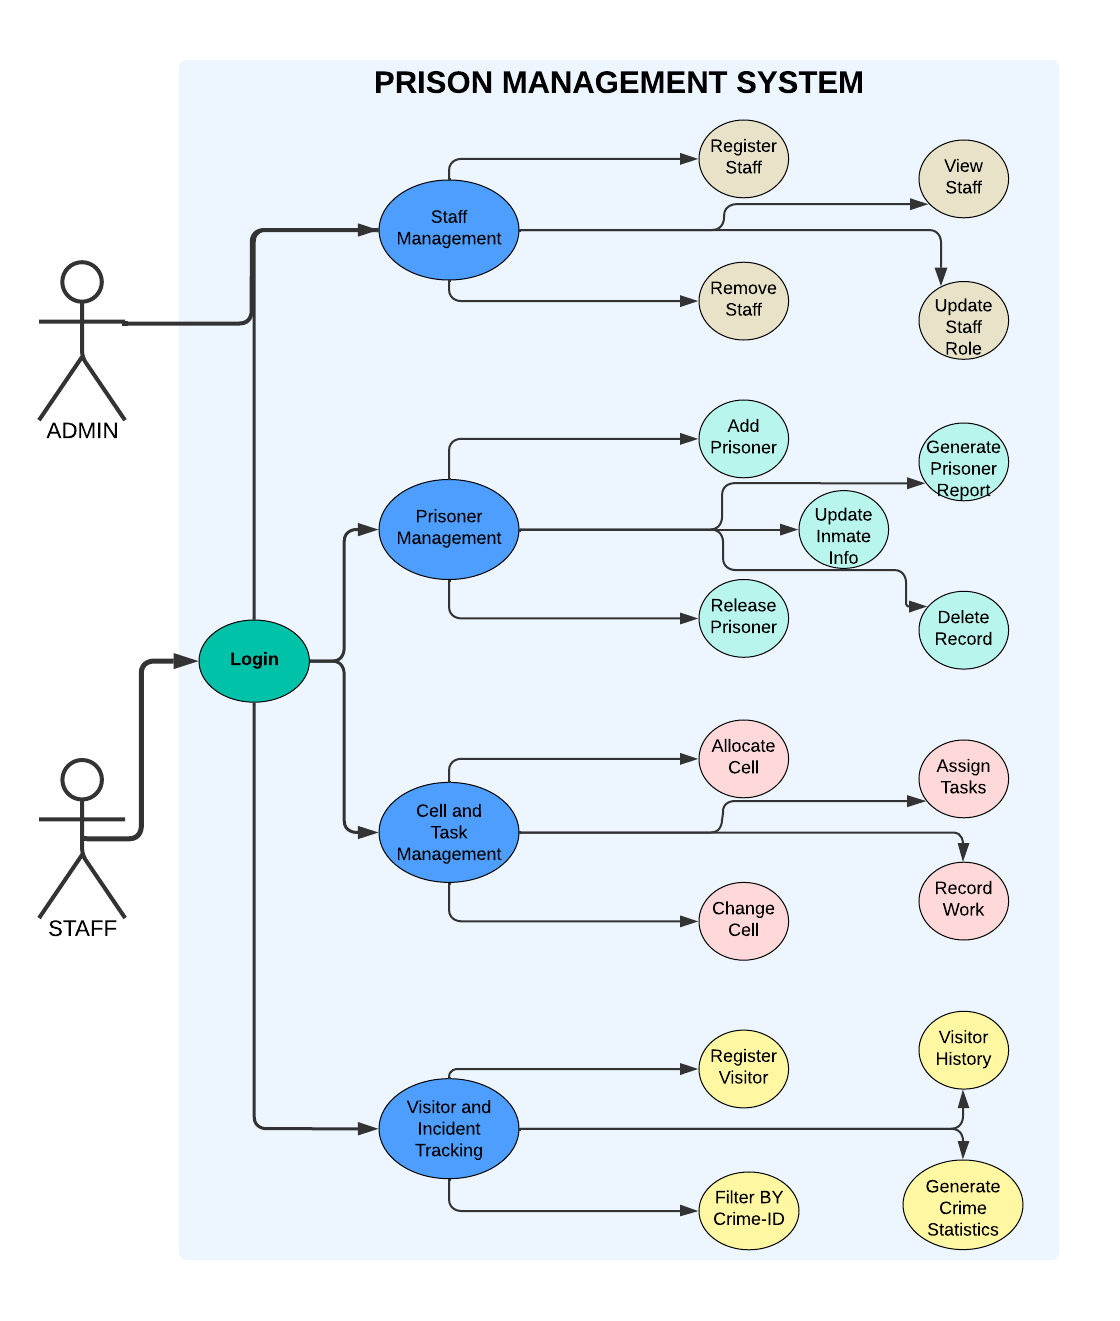
\includegraphics[width=0.7\textwidth,height=0.85\textheight]{usecase.png}
        \caption{3.2.1 Use-Case Diagram}
        \label{fig:use-case}
    \end{figure}
\end{frame}
\begin{frame}{} %Class Diagram
    \begin{figure}
        \centering
        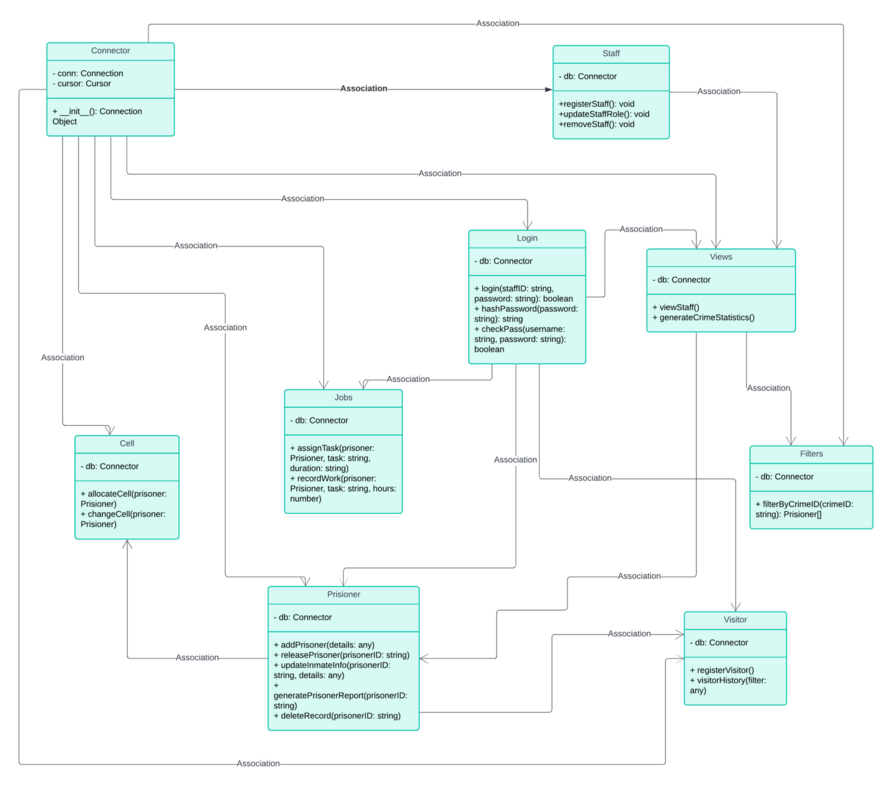
\includegraphics[width=0.5\linewidth]{class3comp.png}
        \caption{3.2.2 Class Diagram}
        \label{fig:class}
    \end{figure}
\end{frame}
\begin{frame}{}%Activity Diagram}
    \begin{figure}
        \centering
        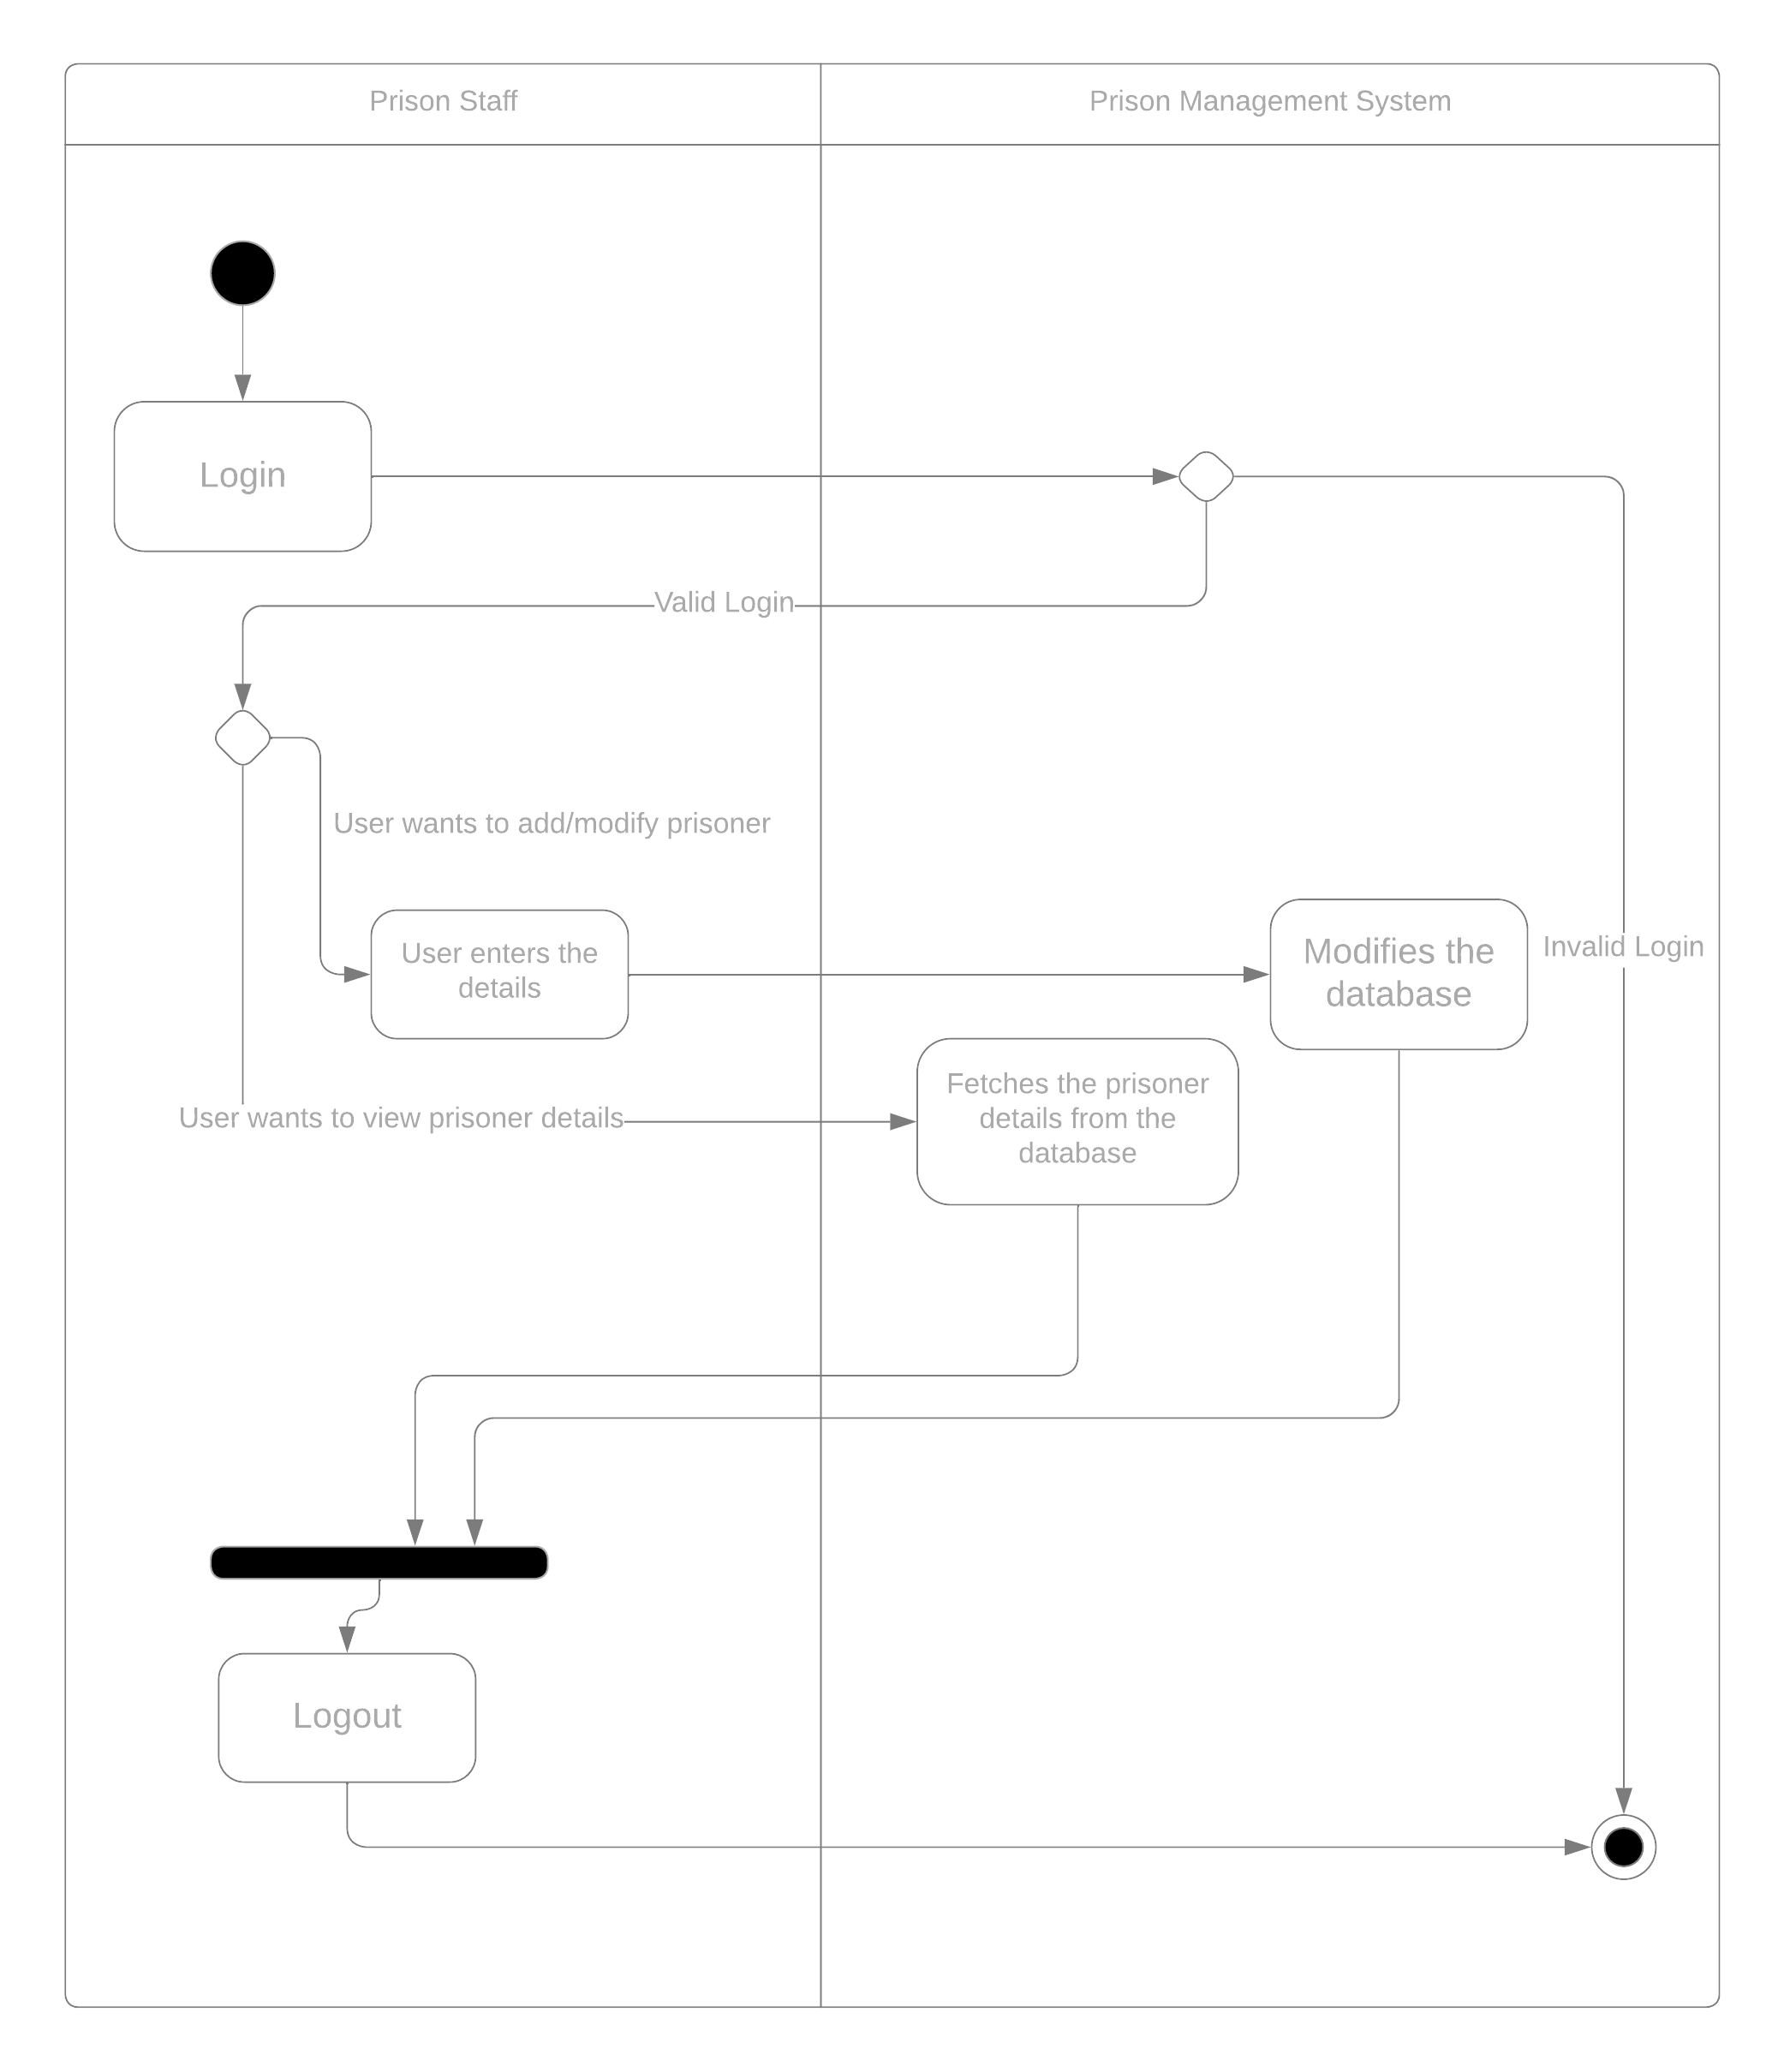
\includegraphics[width=0.5\linewidth,height=0.85\textheight]{activity.png}
        \caption{3.2.3 Activity Diagram}
        \label{fig:activity}
    \end{figure}
\end{frame}

\begin{frame}{}%Sequence Diagram}
    \begin{figure}
        \centering
        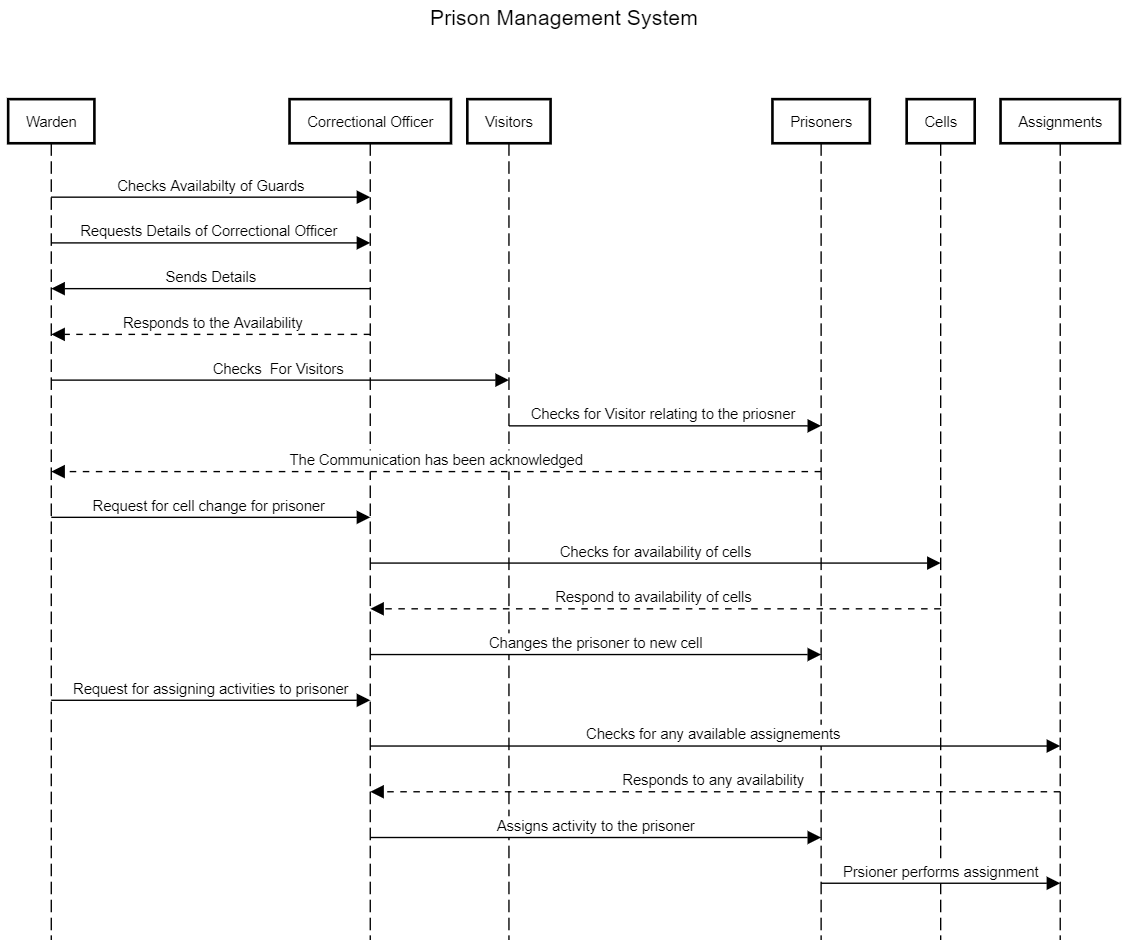
\includegraphics[width=0.5\linewidth,height=0.85\textheight]{sequence.png}
        \caption{3.2.4 Sequence Diagram}
        \label{fig:sequence}
    \end{figure}
\end{frame}
\begin{frame}{}%ER Diagram}
    \begin{figure}
        \centering
        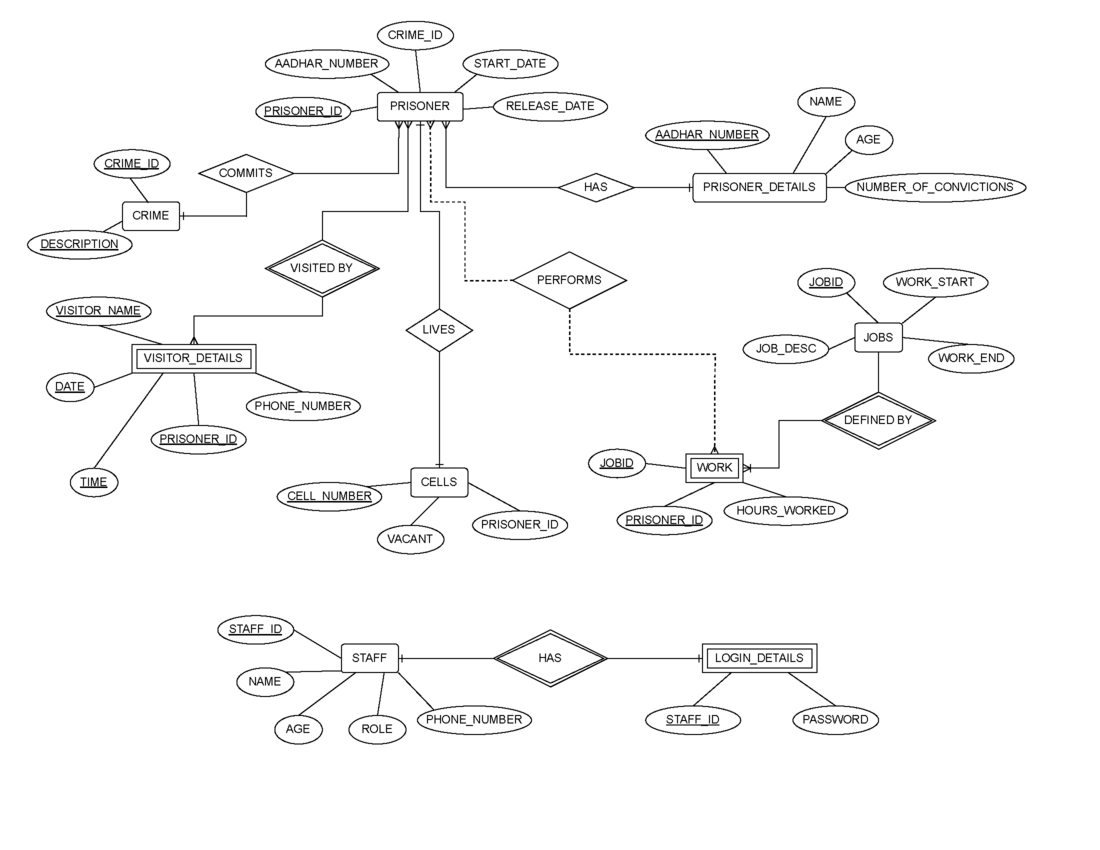
\includegraphics[width=0.7\linewidth,height=0.87\textheight]{ercomp.png}
        \caption{3.2.5 ER Diagram}
        \label{fig:er}
    \end{figure}
\end{frame}
\section{Result Screenshots}
\begin{frame}{Screenshots}
    \begin{figure}
        \centering
        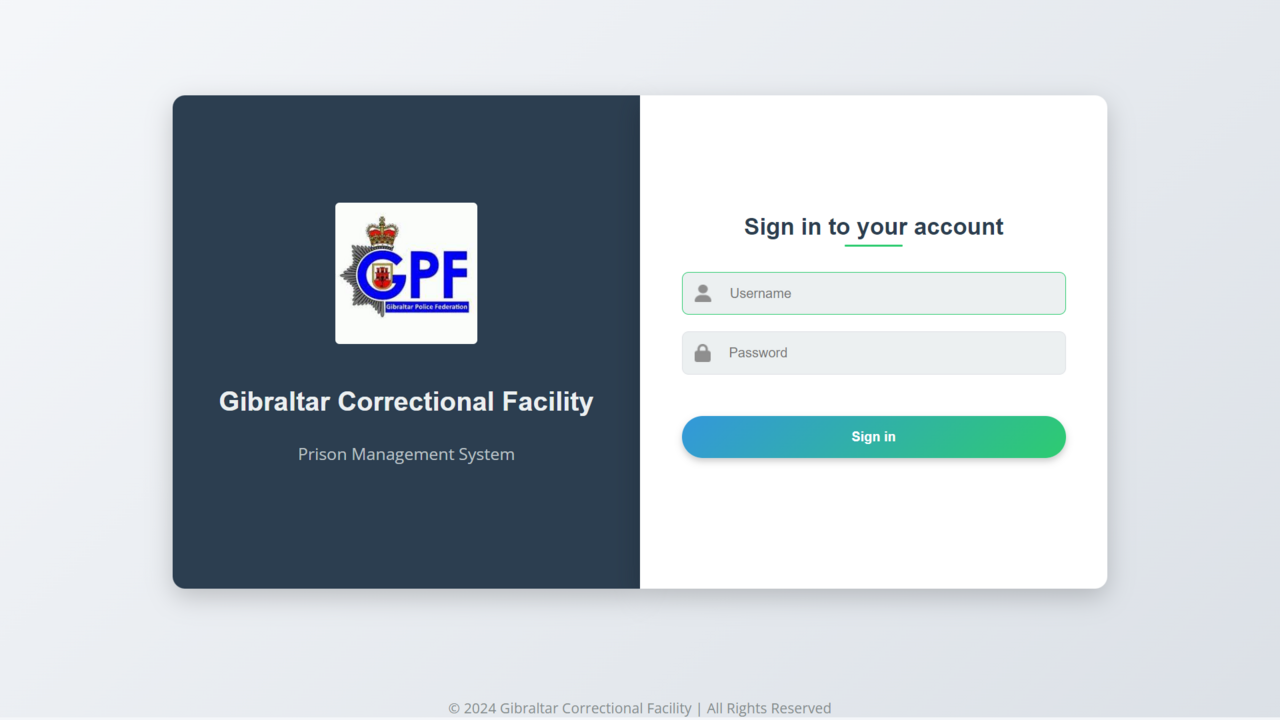
\includegraphics[width=0.6\linewidth]{login.png}
        \caption{4.1 Login Screen}
        \label{fig:login}
    \end{figure}
\end{frame}
\begin{frame}{Screenshots}
    \begin{figure}
        \centering
        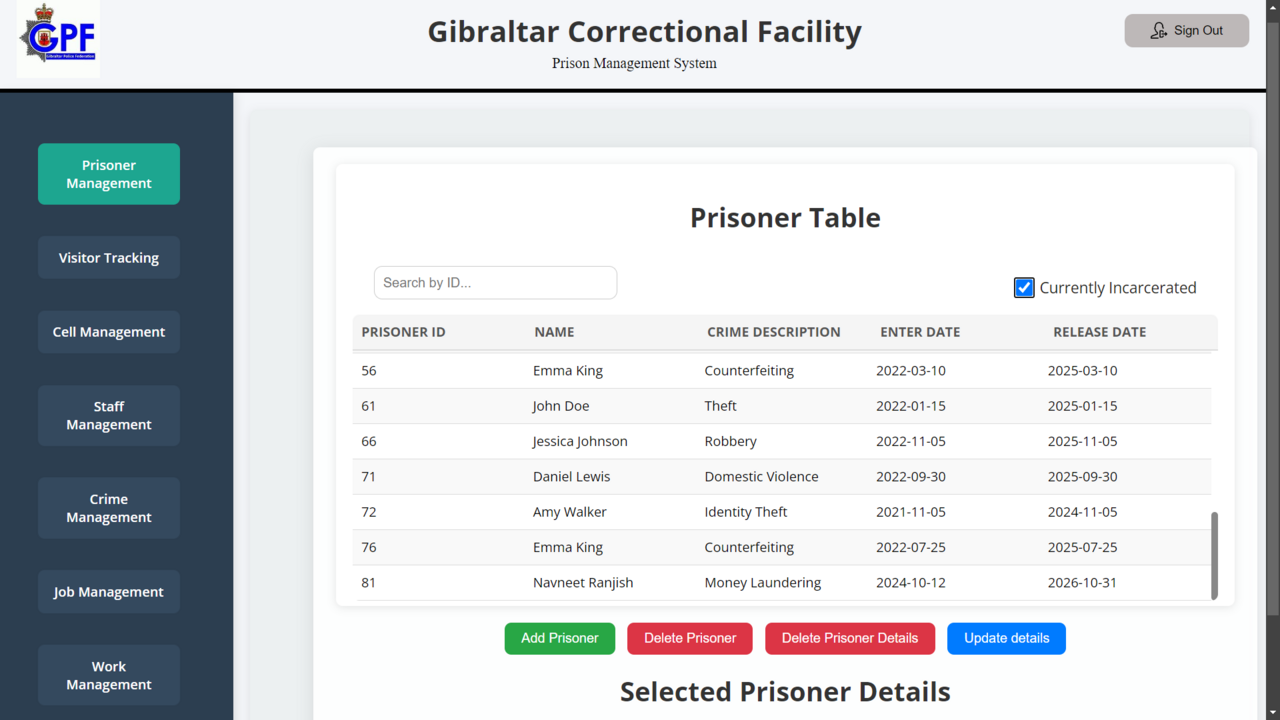
\includegraphics[width=0.6\linewidth]{prisonermgmt.png}
        \caption{4.2 Prisoner Management}
        \label{fig:pmgmt}
    \end{figure}
\end{frame}
\begin{frame}{Screenshots}
    \begin{figure}
        \centering
        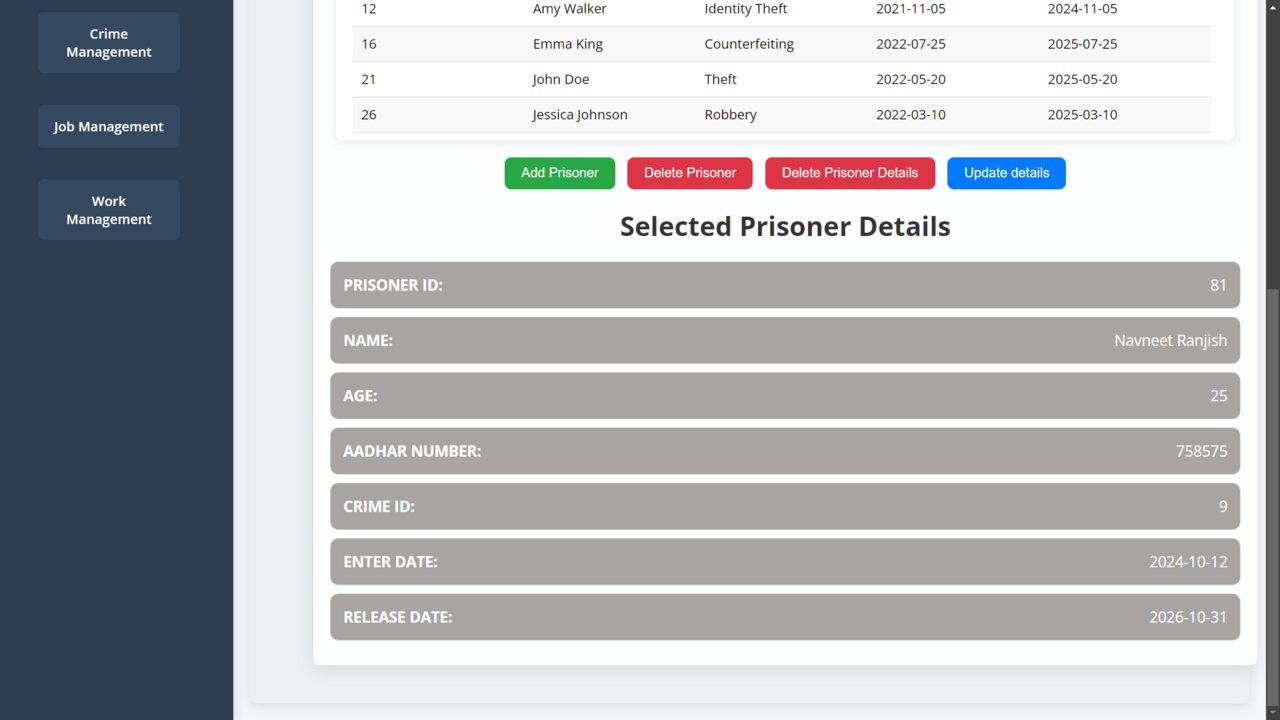
\includegraphics[width=0.6\linewidth]{prisonerdet.png}
        \caption{4.3 Prisoner Details}
        \label{fig:pdet}
    \end{figure}
\end{frame}
\begin{frame}{Screenshots}
    \begin{figure}
        \centering
        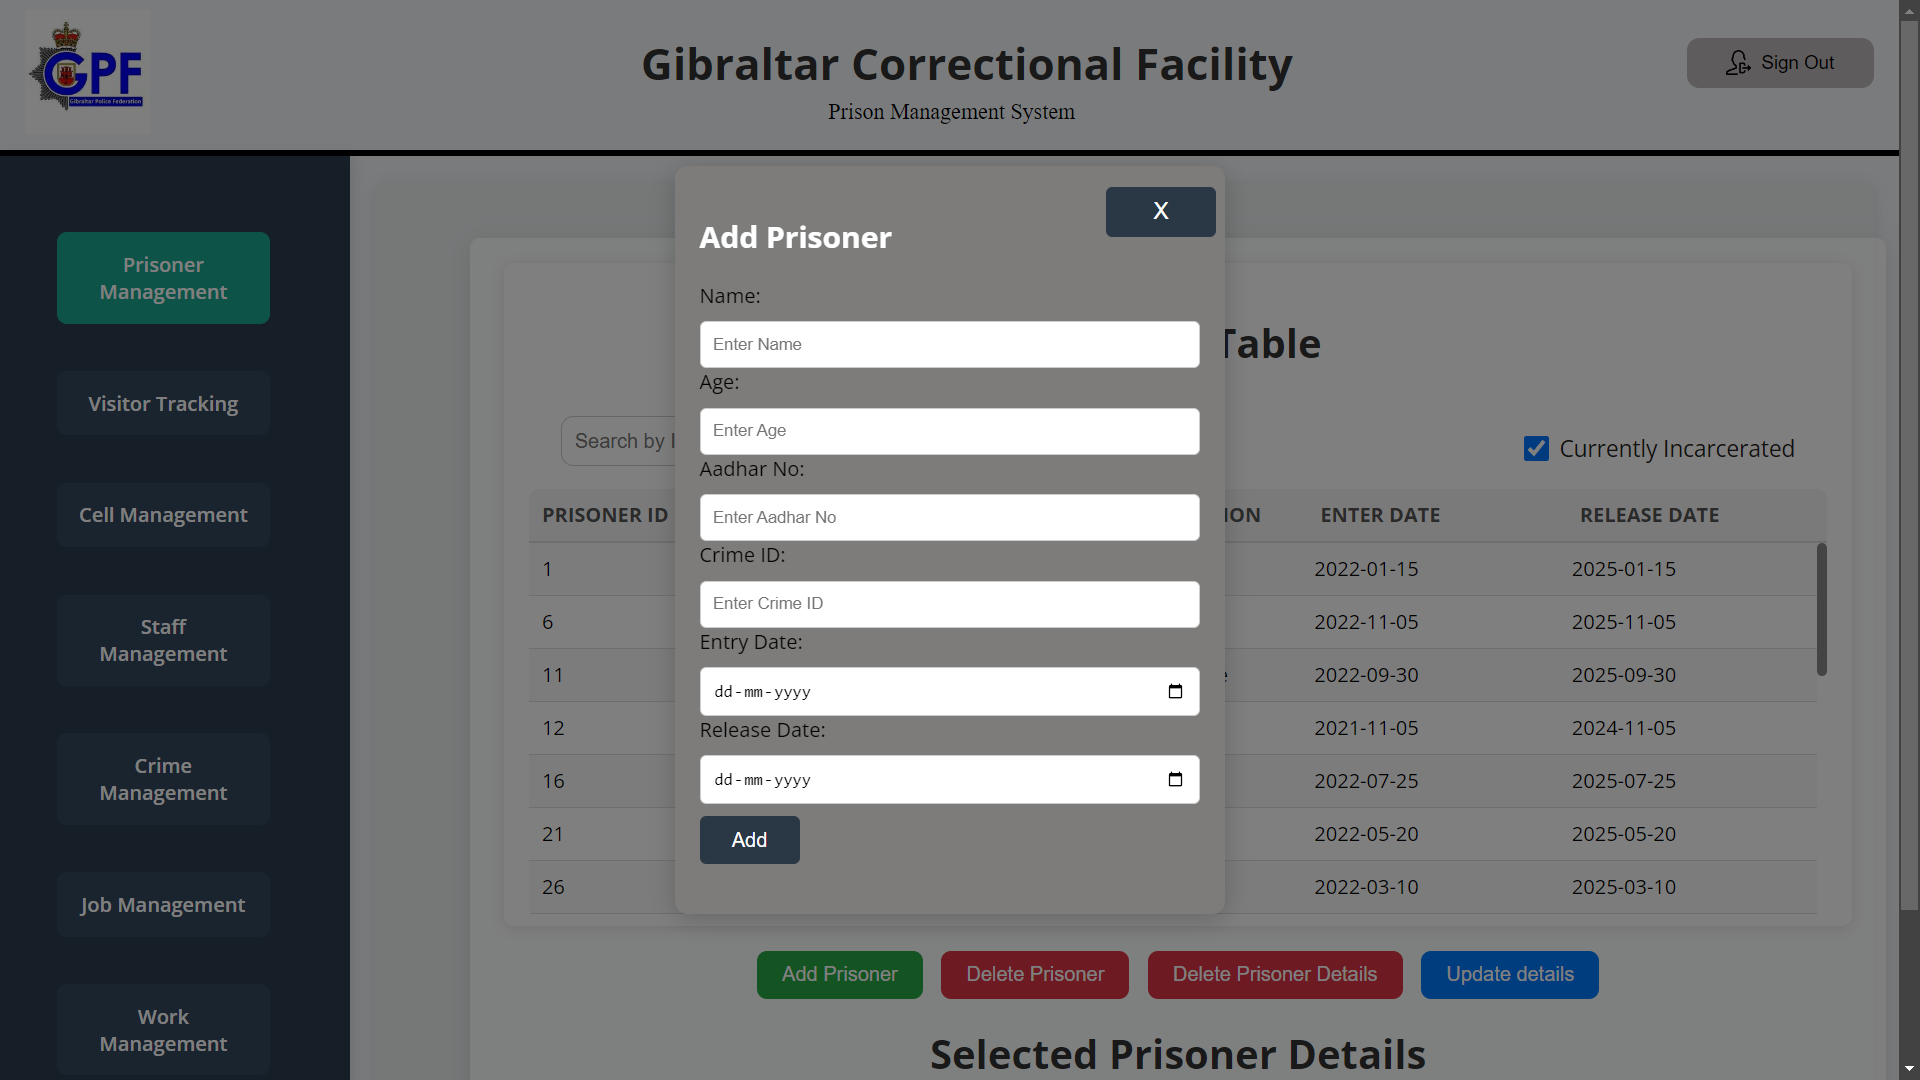
\includegraphics[width=0.6\linewidth]{addprisoner.png}
        \caption{4.4 Add Prisoner Dialog}
        \label{fig:addp}
    \end{figure}
\end{frame}
\begin{frame}{Screenshots}
    \begin{figure}
        \centering
        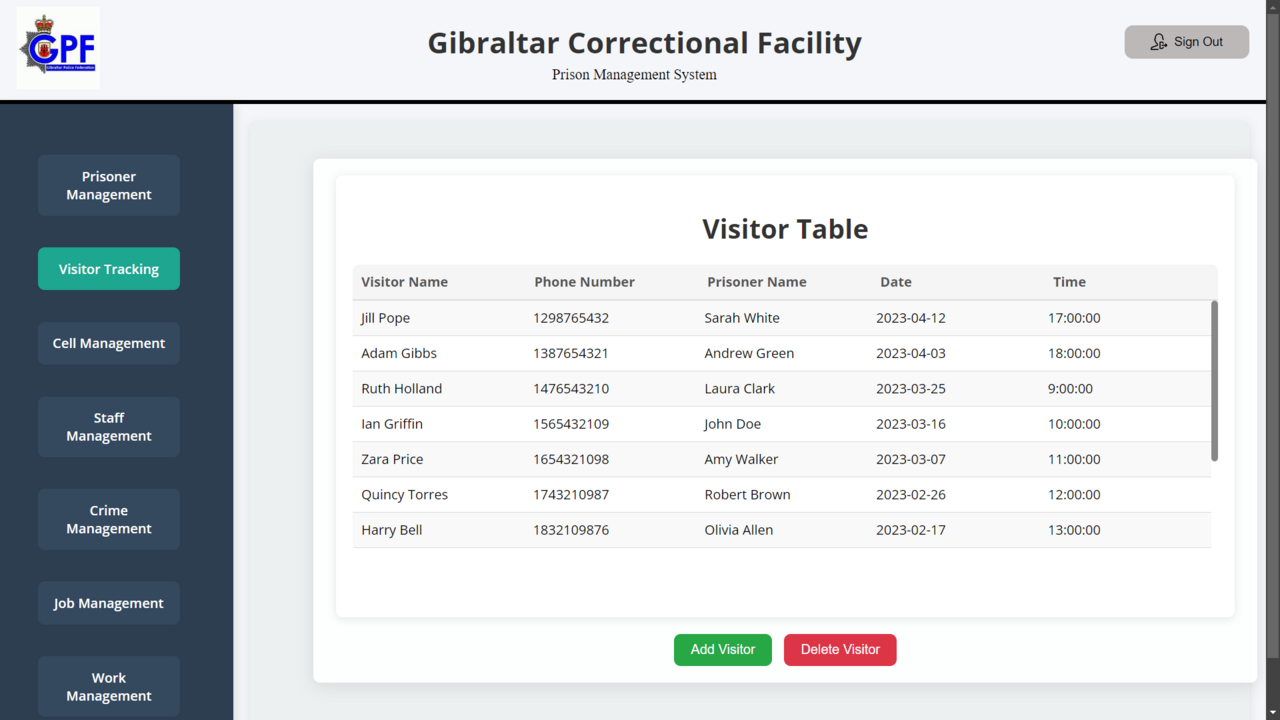
\includegraphics[width=0.6\linewidth]{visitor.png}
        \caption{4.5 Visitor Management}
        \label{fig:visitor}
    \end{figure}
\end{frame}
\begin{frame}{Screenshots}
    \begin{figure}
        \centering
        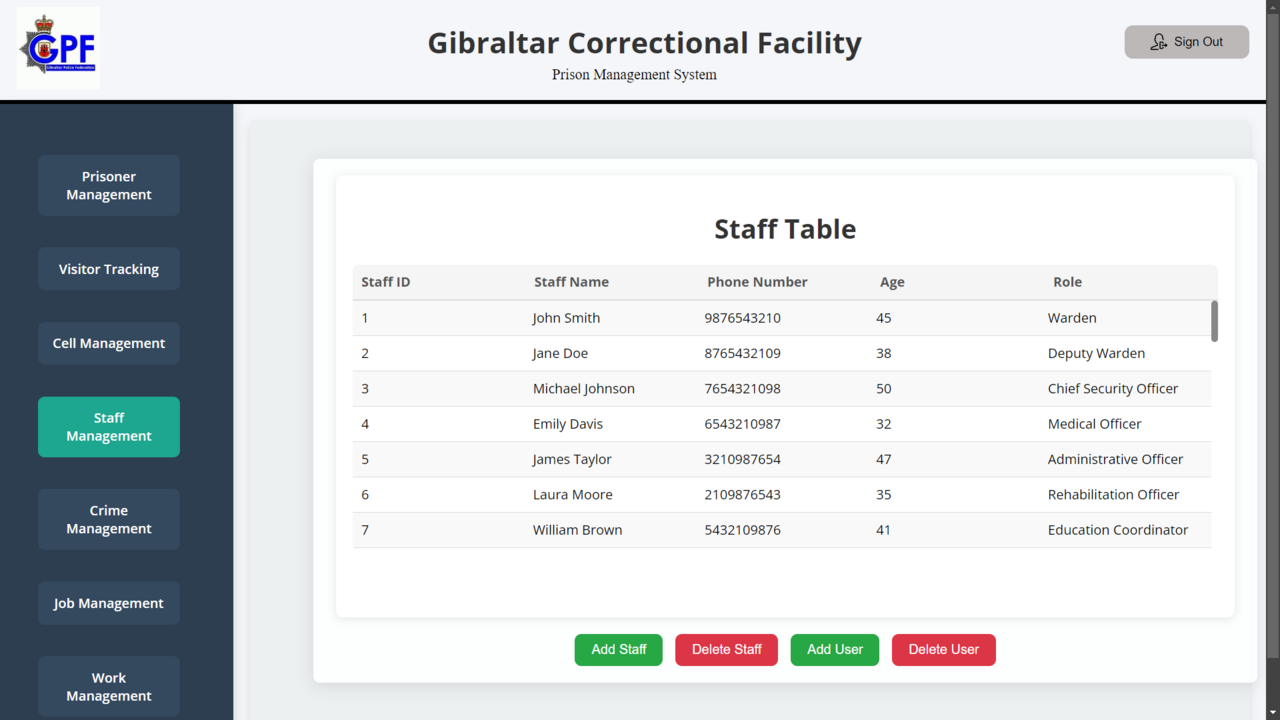
\includegraphics[width=0.6\linewidth]{staff.png}
        \caption{4.6 Staff Management}
        \label{fig:staff}
    \end{figure}
\end{frame}
\begin{frame}{Screenshots}
    \begin{figure}
        \centering
        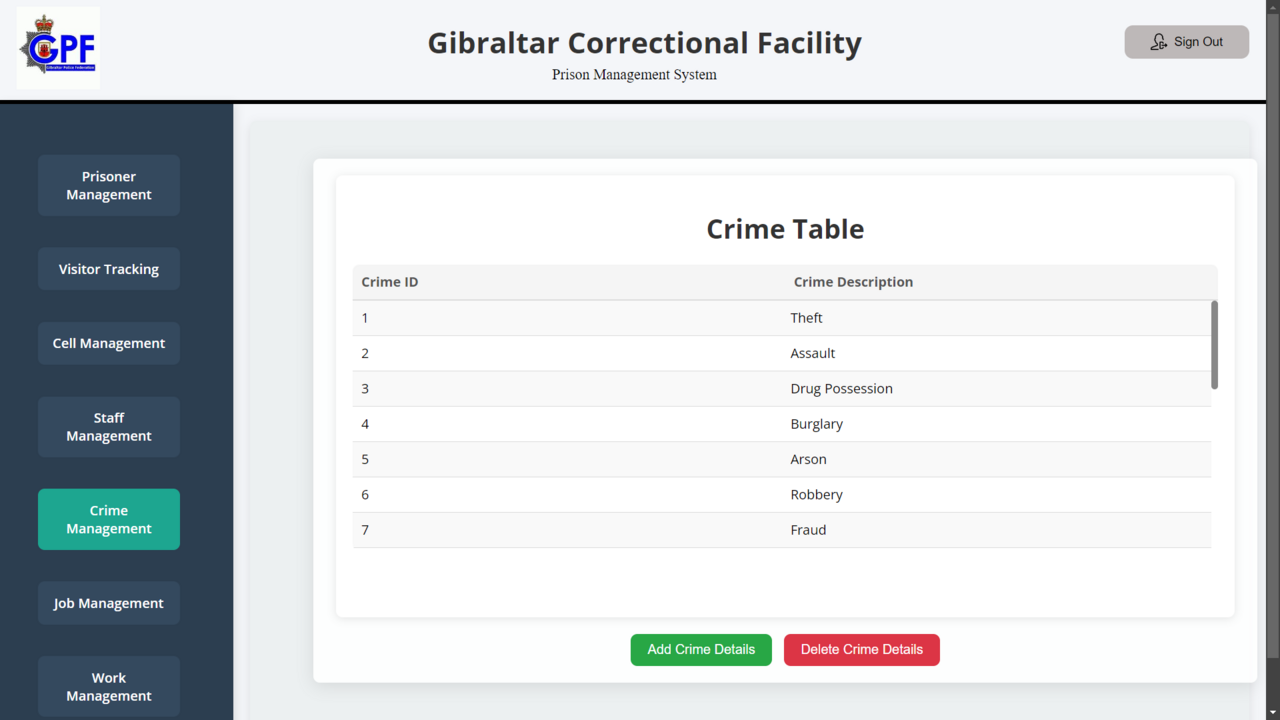
\includegraphics[width=0.6\linewidth]{crime.png}
        \caption{4.7 Crime Management}
        \label{fig:crime}
    \end{figure}
\end{frame}
\begin{frame}{Screenshots}
    \begin{figure}
        \centering
        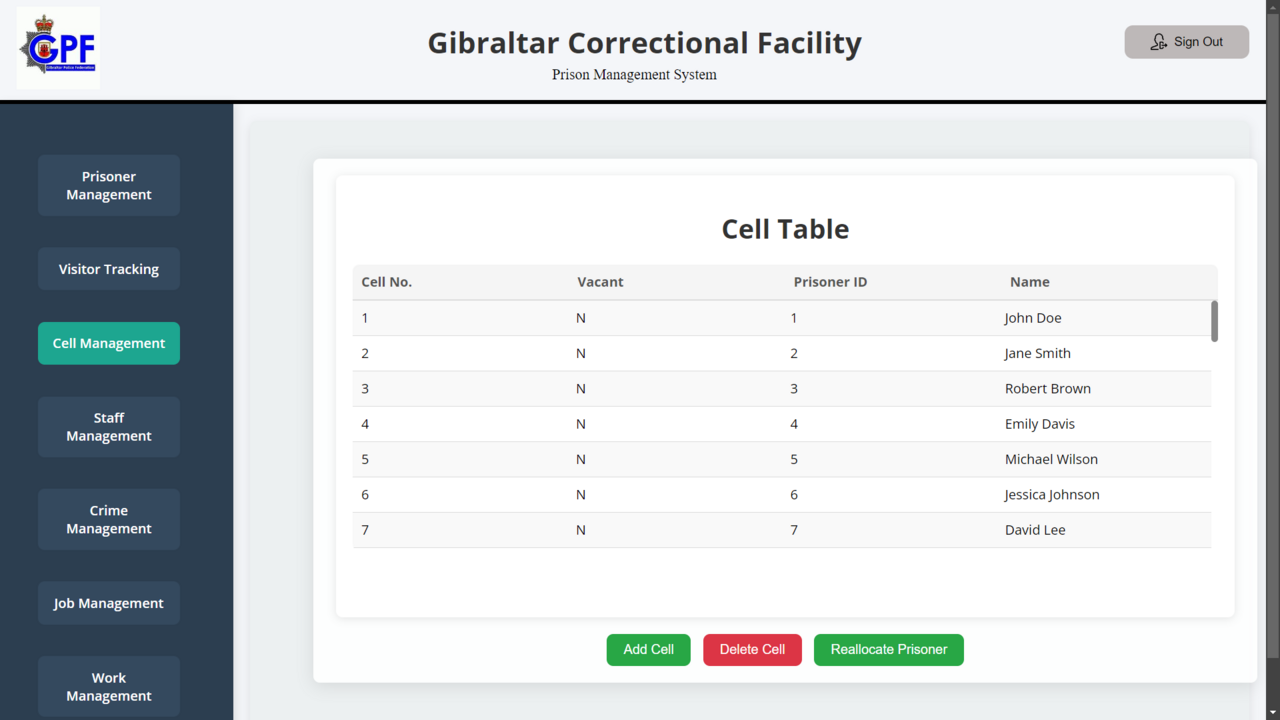
\includegraphics[width=0.6\linewidth]{cell.png}
        \caption{4.8 Cell Management}
        \label{fig:cell}
    \end{figure}
\end{frame}
\begin{frame}{Screenshots}
    \begin{figure}
        \centering
        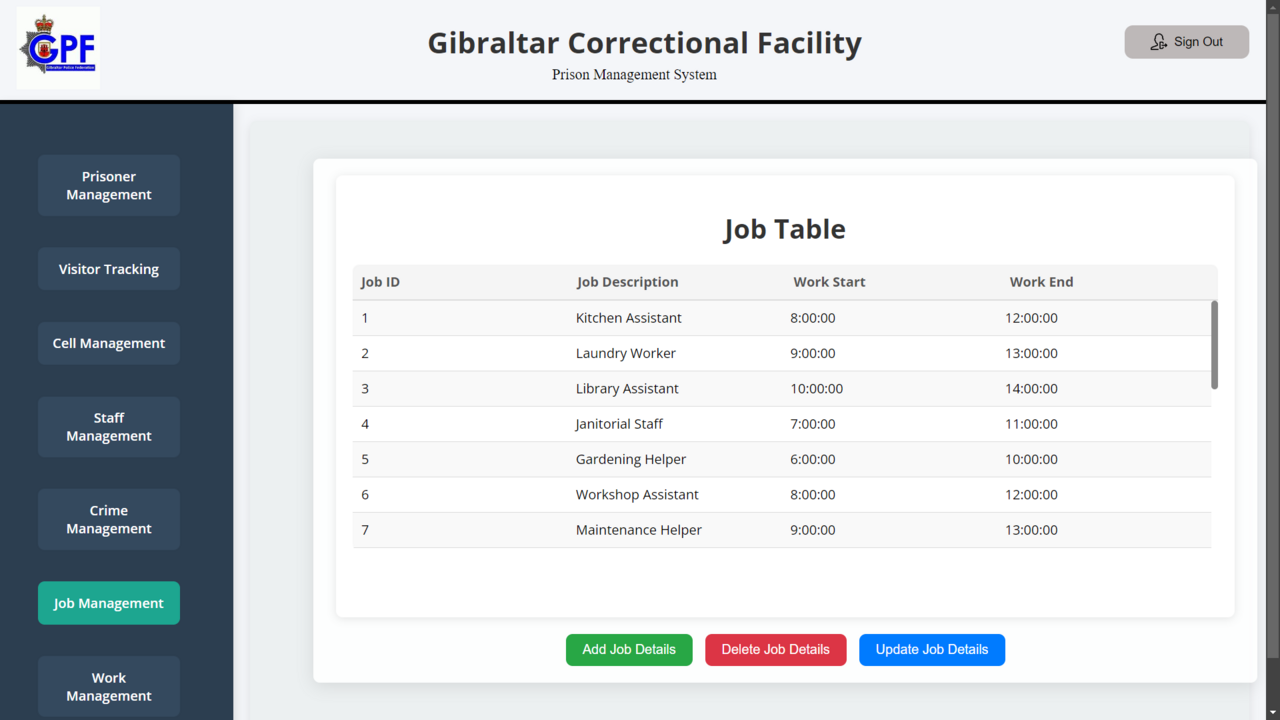
\includegraphics[width=0.6\linewidth]{job.png}
        \caption{4.9 Job Management}
        \label{fig:job}
    \end{figure}
\end{frame}
\begin{frame}{Screenshots}
    \begin{figure}
        \centering
        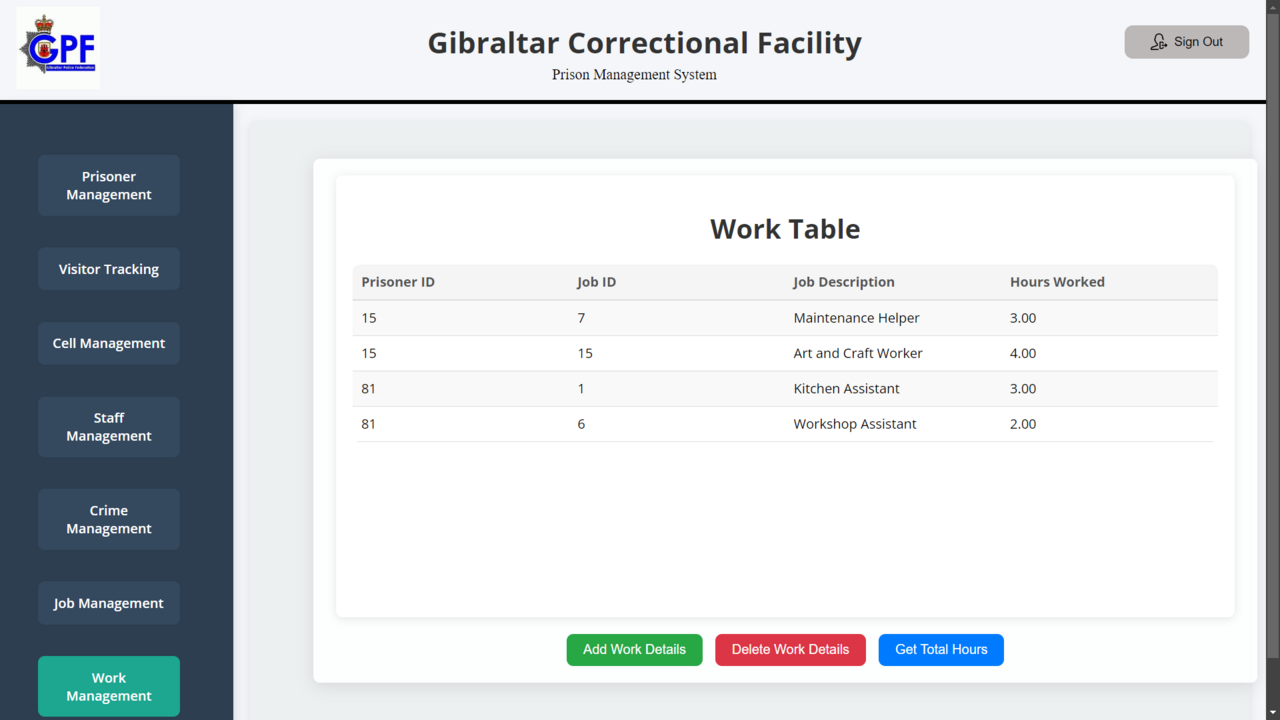
\includegraphics[width=0.6\linewidth]{work.png}
        \caption{4.10 Work Management}
        \label{fig:work}
    \end{figure}
\end{frame}

\section{References}
\begin{frame}{References}
    \printbibliography
    
\end{frame}

\end{document}